\RequirePackage[T1]{fontenc}
\documentclass[conference]{IEEEtran}
\usepackage{amsmath,amssymb}
\usepackage{booktabs}
\usepackage{graphicx}
\usepackage[hidelinks]{hyperref}
\usepackage{cite}
\graphicspath{{figures/}}

\title{Reinforcement Learning with Verifiable Rewards\\for Mathematical Reasoning: A Controlled Empirical Study}
\author{
\IEEEauthorblockN{Tuan Minh Pham, Tri Vo, Yahor Lechanka}
\IEEEauthorblockA{Purdue University\\CS 557 -- Final Project Report Draft}
}

\begin{document}
\maketitle

\begin{abstract}
We study how reinforcement learning with verifiable rewards changes mathematical answer accuracy, exploration, and response efficiency. Starting from Qwen2.5-Math-1.5B, we compare GRPO and Dr.~GRPO with an unchanged model and a supervised fine-tuning control. Both RL configurations improve competition-math and arithmetic benchmark performance under a shared evaluation protocol. Controlled tables examine learning rate, KL regularization, clipping, reward design, training exploration and decoding settings. Higher update strength helps within the tested range, whereas the tested format and length rewards do not improve greedy development accuracy. Longer GRPO training improves sampled reliability and external benchmark accuracy despite reducing original-prompt greedy development accuracy. Dense training curves and discrete held-out measurements distinguish optimization progress from generalization. Prompt wording and answer-selection rules alter the interpretation of checkpoint quality, and their gains must be weighed against inference cost. Our implementation validates restart equivalence across training segments and dataset passes.
\end{abstract}

\section{Introduction}
Mathematical problem solving offers a useful setting for studying reinforcement learning (RL) because many tasks provide verifiable final answers. A policy can generate alternative solutions, receive correctness feedback, and update without imitating one reference derivation. This creates an opportunity to study not only whether post-training improves answers, but also what changes: reliable deterministic decoding, success under sampling, completion behavior, or the range of problems solved.

These outcomes need not move together. A higher training reward can reflect better fit to repeated training problems. A higher sampled success rate can indicate more reliable responses on already-solvable questions, rather than an expanded set of solvable questions. A shorter response can be efficient or prematurely incomplete. Consequently, an evaluation based only on final accuracy or training loss can miss important aspects of RL adaptation.

We investigate these distinctions with Qwen2.5-Math-1.5B~\cite{qwen}, competition mathematics from MATH~\cite{math}, and an arithmetic transfer check on GSM8K~\cite{gsm8k}. We focus on GRPO and Dr.~GRPO under shared initialization, training data, prompts and grading. Separate controlled studies examine optimization hyperparameters, reward design, exploration settings and training duration. A matched-data supervised fine-tuning (SFT) run provides an additional control.

The completed study establishes four main findings. First, both RL configurations improve external mathematical accuracy relative to the unchanged base, with GRPO increasing MATH-500 accuracy from 34.8\% to 67.4\% in the initial comparison. Second, learning-rate tuning improves the reference GRPO configuration, whereas the tested KL and clipping changes do not. Third, adding format or length rewards does not improve greedy development accuracy, although the length penalty shortens responses. Fourth, longer tuned GRPO training improves sampled pass@1 and external accuracy while reducing original-prompt greedy development accuracy. At 512 updates, MATH-500 reaches 70.4\% and GSM8K-100 reaches 85.0\%. Both decoding rule and evaluation distribution therefore change the interpretation of progress.

The contribution is a controlled empirical comparison and a reproducible implementation, not a new optimization algorithm or a reproduction of a large-scale reasoning-model recipe. The completed runs use 512 training problems; larger-data and longer-update stages of the project plan remain future experiments. The presentation uses one fixed reference run per ablation, without cross-run averaging or selecting a different run for each favorable outcome.

\section{Background and Research Questions}
\subsection{Outcome-Verified Policy Learning}
Let $x$ denote a mathematical problem, $y$ a generated solution, and $a$ the reference answer. Our correctness reward is
\begin{equation}
C(x,y)=\mathbf{1}\!\left[\operatorname{equiv}(\operatorname{extract}(y),a)\right].
\end{equation}
The extractor identifies the final answer; normalized exact matching and mathematical-equivalence checks determine correctness. Missing or ungradable answers receive zero. This reward verifies an outcome, not every intermediate reasoning step. A correct final answer therefore does not establish a valid proof.

SFT instead optimizes the likelihood of a reference solution. RL learns from the model's own sampled responses and can reward a correct alternative to that reference. The distinction motivates comparing both methods, but does not imply that RL must outperform a well-tuned SFT recipe.

\subsection{Peer Optimization Methods}
GRPO~\cite{grpo} compares responses sampled for the same problem. A typical group-relative advantage is
\begin{equation}
A_i=\frac{r_i-\overline{r}}{s_r+\varepsilon},
\end{equation}
where $\overline{r}$ and $s_r$ are the group's reward mean and standard deviation. Dr.~GRPO~\cite{drgrpo} removes the group-standard-deviation scaling and uses a fixed token-loss denominator. This comparison isolates two practical choices in group-relative optimization: reward scaling and response-length normalization.

The two configurations share the starting model and training data. Each backend is configured explicitly and checked against its intended loss and gradient behavior; the subsequent hyperparameter and reward studies use GRPO as the fixed reference optimizer.

\subsection{Questions}
The study asks: (1) How do GRPO and Dr.~GRPO compare with no training and SFT? (2) Which optimization settings improve held-out accuracy? (3) Do extra reward components improve correctness or merely alter output form and length? (4) How do training sampling and additional updates change greedy accuracy, sampled reliability and observed coverage? (5) Can the training trajectory be continued reproducibly across separate execution segments?

\section{Experimental Design}
\subsection{Initialization, Data, and Controls}
All main experiments start from the same Qwen2.5-Math-1.5B \emph{base} checkpoint. RL and SFT update the full model. The unchanged base uses the same problem presentation as the trained models. Historical 7B, retrieval, verifier-selection, and adapter experiments are not combined with this matched 1.5B comparison.

We freeze 512 eligible MATH training problems at difficulty Levels 3--5. Before training selection,300 disjoint, category/level-balanced examples from MATH train are reserved for development. Stable source IDs and normalized problem hashes identify the split. Reference solutions are available only as grading references or SFT targets, not as demonstrations in RL prompts.

External evaluation uses all 500 MATH-500 problems and a fixed, seeded 100-question GSM8K test subset. Normalized-text overlap with the selected 512 training problems is zero. These benchmark sets were inspected in earlier project work and are not an untouched confirmation set; pretraining contamination is unknown. Development results guide tuning, while external scores are reported separately.

\subsection{Training Protocol}
The initial method comparison uses 128 optimizer updates, one pass over 512 unique problems and learning rate $10^{-6}$. Each rollout batch contains 16 problems with four sampled responses each. Four optimizer updates consume the resulting 64 responses. Sampling uses temperature 1, top-$p=1$ and no top-$k$ cutoff. Prompt and completion limits are 1024 and 3000 tokens. The learning rate is constant, the initial KL coefficient is zero, and AdamW uses the same settings across methods. FP32 trainable weights with BF16 compute are used uniformly; this is full-parameter training, not LoRA.

GRPO and Dr.~GRPO use lower/upper clipping distances 0.2/0.2. The comparison holds other optimization settings fixed; these are evaluated pilot configurations, not globally optimized recipes.

The SFT control starts from the same base and uses the same 512 problem IDs with ground-truth solution targets. It applies assistant-only cross-entropy using the same chat prefix, one epoch, and a separate conservative learning rate. SFT and RL are matched by training data, not by token cost or optimization effort; the SFT control has not received the same tuning study.

\subsection{Evaluation and Exploration}
Greedy evaluation produces one deterministic completion per problem. Sampled evaluation generates eight responses for each of 100 fixed development problems at temperature 1. If $c$ of $n=8$ responses are correct, we estimate
\begin{equation}
\widehat{\operatorname{pass@}k}=1-\frac{\binom{n-c}{k}}{\binom{n}{k}},
\end{equation}
with the numerator zero when $n-c<k$. Sampled pass@1 estimates the accuracy of a sampled response; it is not greedy accuracy. Pass@8 measures observed oracle coverage, not the accuracy of an answer-selection procedure.

All comparisons use a common final-answer grader and evaluation stopping convention accepting both end-of-text and chat-end tokens. We record raw responses, source IDs, prompts, token counts, truncation and runtime. The stopping-control audit left the no-RL, GRPO and Dr.~GRPO accuracies unchanged; the SFT score changed slightly to 40.3\%. Thus the main RL gains are not artifacts of changing the stopping rule in that audit. Hyperparameter settings and sparse held-out evaluations are presented as tables, not interpolated learning curves.

Training reward, policy loss, entropy, completion length, and clipping activity are logged separately from held-out scores. GRPO's policy-surrogate loss is not SFT cross-entropy: negative or near-zero scalar losses do not imply that parameter updates have stopped.

\section{Initial Method Comparison}
\begin{table*}[t]
\centering
\caption{Matched GRPO/Dr.~GRPO comparison with no-RL and SFT controls. Greedy accuracy (\%); sampled metrics use 100 fixed problems and eight responses. RL: LR $10^{-6}$,128 updates. SFT external/sampling entries were not evaluated. MATH tokens are mean greedy completion length.}
\label{tab:methods}
\footnotesize
\setlength{\tabcolsep}{4pt}
\begin{tabular}{lrrrrrr}
\toprule
Method & Dev300 & MATH-500 & GSM8K-100 & Sampled@1 & Pass@8 & MATH tokens\\
\midrule
No RL & 45.0 & 34.8 & 38.0 & 29.38 & 79.0 & 1665\\
SFT & 40.3 & --- & --- & --- & --- & ---\\
GRPO & 72.3 & 67.4 & 73.0 & 55.00 & 89.0 & 663\\
Dr.~GRPO & 68.3 & 65.2 & 75.0 & 52.62 & 90.0 & 646\\
\bottomrule
\end{tabular}
\end{table*}

\begin{figure*}[t]
\centering
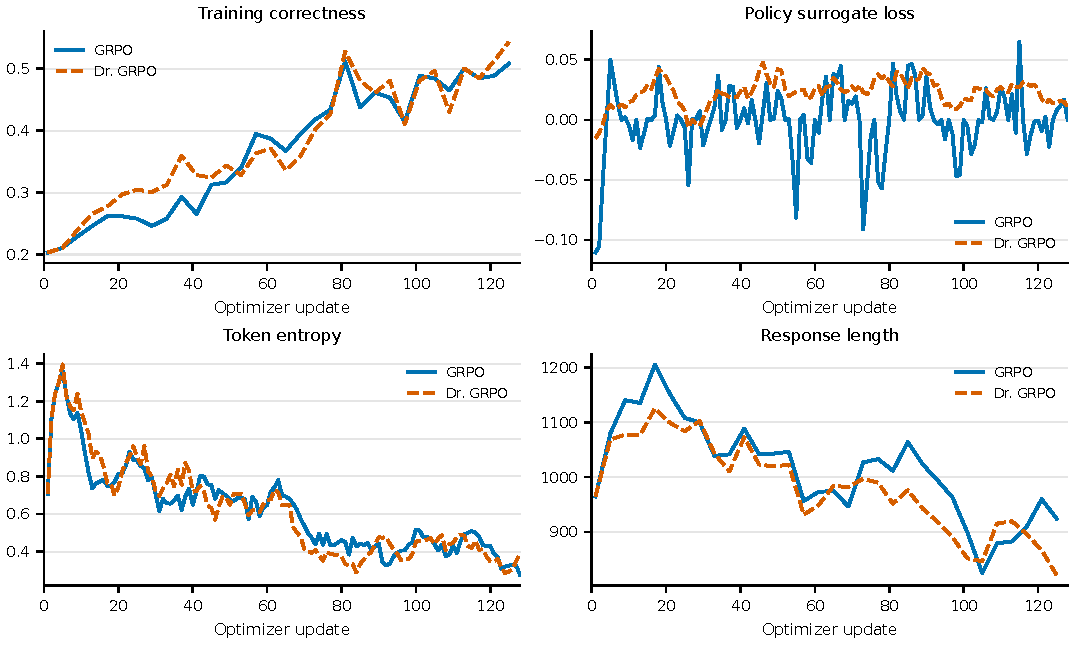
\includegraphics[width=\textwidth]{method_dynamics.pdf}
\caption{Dense training diagnostics for GRPO and Dr.~GRPO at LR $10^{-6}$. Reward and response length use trailing four-observation means; loss and entropy use eight updates. These are logged training measurements, not held-out accuracy or proof-quality curves. The unchanged model has no optimizer-update trajectory.}
\label{fig:methods}
\end{figure*}

\subsection{Accuracy Gains and Transfer}
Table~\ref{tab:methods} shows improvements for both RL configurations. GRPO reaches 72.3\% development accuracy versus 45.0\% without RL, a 27.3-point gain. On MATH-500, the unchanged model scores 34.8\%, compared with 67.4\% for GRPO and 65.2\% for Dr.~GRPO. Dr.~GRPO reaches 75.0\% on GSM8K-100, compared with 38.0\% without RL.

These reference-run results support the effectiveness of the tested settings, not a universal ordering of the algorithms. GRPO's MATH-500 result includes 184 fixed and 21 broken examples relative to the unchanged model, illustrating that the gain is substantial but not uniform across questions.

\subsection{Sampling and Response Efficiency}
Initial sampled pass@8 increases from 79\% without RL to 89\% with GRPO and 90\% with Dr.~GRPO. GRPO's sampled pass@1 rises from 29.38\% to 55.0\%; the substantial difference between greedy and sampled scores reinforces the need to name the decoding rule. These discrete measurements are included in Table~\ref{tab:methods} rather than drawn as a three-point curve.

On MATH-500, GRPO reduces mean completion length from 1664.6 to 662.7 tokens, approximately 60\%, while improving answer accuracy. Truncation falls from 209/500 to 12/500. Similar completion improvements occur on GSM8K-100. These outcomes demonstrate improved accuracy and practical completion efficiency under the shared budget; they do not establish that shortening itself causes the accuracy gain. The unchanged model's high truncation rate is part of its measured behavior under this fixed cap, not a reason to suppress its outcome.

The SFT control scores 40.3\% on dev 300. It does not reproduce the RL gains in this initial configuration. Because SFT is not compute-matched or comparably tuned, this is a control result rather than a broad claim against supervised adaptation. External and sampled SFT scores were not collected and are shown as missing, not zero.

\section{Optimization Ablations}
\begin{table*}[t]
\centering
\caption{One-factor learning-rate sweep: dev 300 accuracy (\%),128 updates, one fixed reference run per condition. Dashes denote unrun settings, not zero accuracy. Other settings remain fixed within each method.}
\label{tab:rates}
\footnotesize
\setlength{\tabcolsep}{4pt}
\begin{tabular}{lrrrrr}
\toprule
Method & $2\cdot10^{-7}$ & $5\cdot10^{-7}$ & $10^{-6}$ & $2\cdot10^{-6}$ & $3\cdot10^{-6}$\\
\midrule
GRPO & 49.3 & 61.7 & 72.3 & 70.0 & 75.0\\
Dr.~GRPO & 51.0 & 63.3 & 68.3 & --- & ---\\
\bottomrule
\end{tabular}
\end{table*}

\begin{table}[t]
\centering
\caption{GRPO regularization at LR $10^{-6}$, one fixed reference run per condition. Prefix KL is an offline shared-context diagnostic, not training KL. Clip fraction is a fraction, not a percentage.}
\label{tab:regularization}
\footnotesize
\setlength{\tabcolsep}{4pt}
\begin{tabular}{lrrr}
\toprule
Setting & Dev300 & Prefix KL & Clip fraction\\
\midrule
Control & 72.3 & 0.0459 & 0.000054\\
$\beta=0.001$ & 70.3 & 0.0316 & 0.000048\\
$\beta=0.01$ & 71.0 & 0.0298 & 0.000052\\
Clip $0.1/0.1$ & 68.7 & 0.0229 & 0.002073\\
Clip $0.3/0.3$ & 70.7 & 0.0426 & 0.000007\\
\bottomrule
\end{tabular}
\end{table}

\subsection{Learning Rate}
The initial lower-rate sweep holds the dataset, reference run, update count and evaluation fixed within each method. GRPO and Dr.~GRPO improve as the rate increases from $2\cdot 10^{-7}$ through $5\cdot 10^{-7}$ to $10^{-6}$ (Table~\ref{tab:rates}). This suggests that update strength is important in the short adaptation budget, without establishing that a larger rate will always be better.

An additional GRPO-only upward sweep gives 70.0\% at $2\cdot 10^{-6}$ and 75.0\% at $3\cdot 10^{-6}$, versus 72.3\% at $10^{-6}$. The response is not monotonic across every tested rate. The fixed-reference results motivate using $3\cdot10^{-6}$ for the subsequent GRPO experiments, without claiming a definitive optimum.

These tuned development scores must not be substituted into the initial benchmark table. That table evaluates LR $10^{-6}$ models, while the latest LR $3\cdot 10^{-6}$ checkpoint benchmarks are tracked separately.

\subsection{KL and Clipping}
At the original LR anchor, tested KL coefficients 0.001 and 0.01 yield 70.3\% and 71.0\%, below 72.3\% without the penalty. Offline fixed-prefix reference KL decreases, but lower drift does not improve greedy development accuracy in these runs. Fixed-prefix KL and sampled training KL are different statistics and are not interchangeable.

Symmetric clipping distances 0.1 and 0.3 yield 68.7\% and 70.7\%, also below the 0.2 control. Clipping is rarely active in the control, so the study does not attribute its gains to frequent clipping. The results motivate retaining the current reference settings while extending the data and training studies, rather than combining independently unhelpful changes.

\section{Reward Design and Training Exploration}
\begin{table}[t]
\centering
\caption{Reward design at LR $3\cdot 10^{-6}$: dev 300 accuracy (\%) and mean completion tokens, using the fixed reference run per condition rather than cross-run averages. Reward-score scales differ.}
\label{tab:rewards}
\footnotesize
\setlength{\tabcolsep}{4pt}
\begin{tabular}{lrr}
\toprule
Reward & Dev300 & Tokens\\
\midrule
Correctness & 75.0 & 722\\
Format bonus & 74.0 & 713\\
Length penalty & 71.3 & 680\\
\bottomrule
\end{tabular}
\end{table}

\begin{table*}[t]
\centering
\caption{Training exploration at LR $3\cdot 10^{-6}$, one reference run per condition. $G$ is training group size and $T$ training temperature. Evaluations use common settings; group-size arms match unique problems, not updates or token cost.}
\label{tab:exploration}
\footnotesize
\setlength{\tabcolsep}{4pt}
\begin{tabular}{lrrrr}
\toprule
Training setting & Greedy & Sampled@1 & Pass@8 & Train M tokens\\
\midrule
Control ($T=1,G=4$) & 75.0 & 65.50 & 91.0 & 1.90\\
$T=0.7$ & 73.3 & 64.25 & 90.0 & 1.75\\
$T=1.3$ & 72.7 & 59.00 & 87.0 & 4.11\\
$G=2$ & 70.3 & 51.00 & 87.0 & 1.02\\
$G=8$ & 71.3 & 70.25 & 91.0 & 3.56\\
\bottomrule
\end{tabular}
\end{table*}

\subsection{Reward Components}
With the optimizer fixed to GRPO LR $3\cdot 10^{-6}$, we compare correctness alone with two shaped rewards:
\begin{align}
R_{\mathrm{format}}&=C+0.10F,\\
R_{\mathrm{length}}&=C-0.05\min(L/3000,1).
\end{align}
Here $F$ indicates one balanced, nonempty, parseable boxed answer and $L$ counts generated completion tokens. A wrong but correctly formatted response can receive the format bonus. Raw correctness remains the evaluation target, and each reward component is logged independently.

In the fixed reference runs, correctness-only greedy accuracy is 75.0\%, compared with 74.0\% for the format bonus and 71.3\% for the length penalty (Table~\ref{tab:rewards}). The format condition loses three correct answers net despite slightly higher training correctness. A larger shaped reward therefore cannot be interpreted as a reasoning improvement.

The length penalty reduces mean greedy completion length from 722 to 680 tokens while accuracy falls from 75.0\% to 71.3\%. This is an efficiency tradeoff rather than an unconditional success. The reward controls support keeping correctness alone as the present reference.

\subsection{Temperature and Group Size}
Training temperature 0.7 yields 73.3\% greedy development accuracy versus 75.0\% at 1.0. Temperature 1.3 yields 72.7\% and uses 2.17 times the training completion tokens, with much lower training correctness. Increasing training exploration indiscriminately is therefore not helpful in this short pilot.

Changing training group size reveals a more nuanced outcome. Eight responses per problem improve sampled pass@1 from 65.5\% to 70.25\% and pass@4 from 86.2\% to 87.4\%, while pass@8 remains 91\%. Greedy accuracy falls to 71.3\%, and training completion-token cost grows by 1.88 times. Two responses per problem give 70.3\% greedy accuracy and 51.0\% sampled pass@1.

The group-size conditions share 512 unique problems but use 64,128 and 256 updates for groups of 2,4 and 8, respectively. They are not update- or compute-matched. The observed sampling benefit should not be attributed solely to group size, nor should it be presented as a free improvement in deterministic answering.

\section{Longer Training: Reliability versus Coverage}
\begin{table*}[t]
\centering
\caption{Longer GRPO training on the same 512 problems at LR $3\cdot 10^{-6}$. Greedy 100 and sampled metrics use the same problems; train tokens are cumulative. Only measured checkpoints are tabulated; all accuracy metrics are percentages.}
\label{tab:duration}
\footnotesize
\setlength{\tabcolsep}{4pt}
\begin{tabular}{lrrrrr}
\toprule
Updates & Greedy300 & Greedy100 & Sampled@1 & Pass@8 & Train M tokens\\
\midrule
128 & 75.0 & 79.0 & 65.50 & 91.0 & 1.90\\
256 & 73.3 & 78.0 & 68.00 & 91.0 & 3.53\\
512 & 69.0 & 74.0 & 73.25 & 90.0 & 6.54\\
\bottomrule
\end{tabular}
\end{table*}

\begin{figure*}[t]
\centering
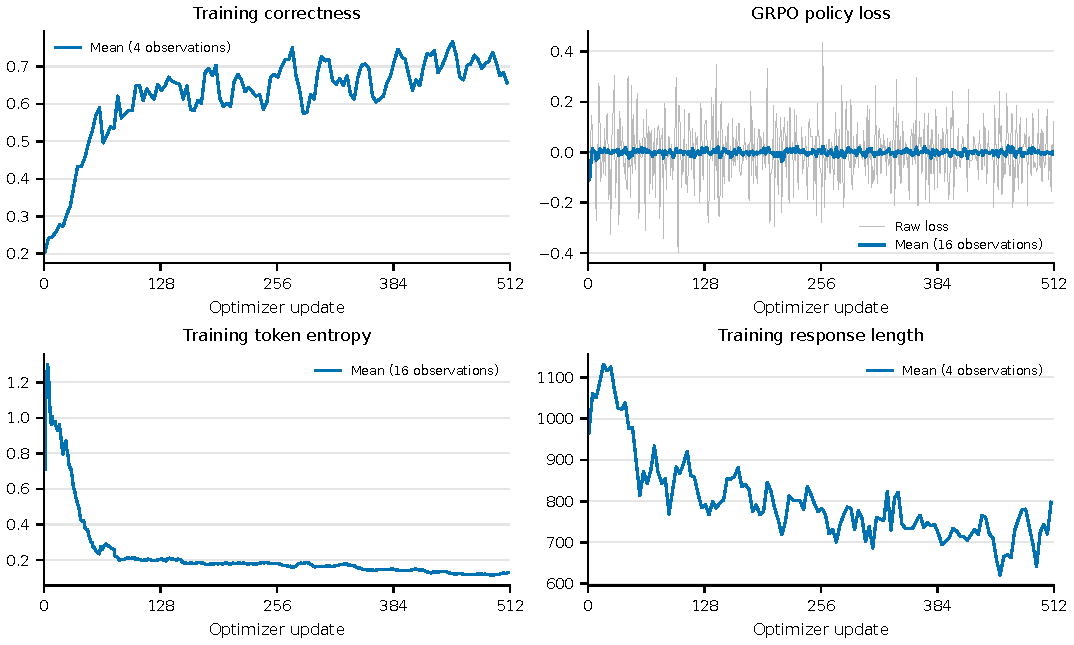
\includegraphics[width=\textwidth]{extended_training.pdf}
\caption{GRPO continuation from 128 to 512 total updates on the same 512 training problems. Reward and length show trailing four-observation means; loss and entropy show 16-update means. Gray loss is raw. The group-relative policy loss can fluctuate around zero while parameters and rewards change; it is not supervised cross-entropy or held-out accuracy.}
\label{fig:extended}
\end{figure*}

Starting from the tuned reference at LR $3\cdot 10^{-6}$, we continue the same optimizer and RNG state to 256 and 512 total updates, corresponding to two and four passes over the same 512 problems. This experiment increases repeated exposure, not training-set diversity. It adds 384 updates to the original 128 rather than training 512 additional updates. Figure~\ref{fig:extended} records dense training dynamics, including policy loss; Table~\ref{tab:duration} separately lists held-out checkpoint measurements.

On-policy training correctness by successive 128-update blocks increases from 50.15\% to 64.31\%,66.31\% and 70.46\%. Nevertheless, greedy dev 300 accuracy falls from 75.0\% to 73.3\% and 69.0\%. The 512-update policy fixes 15 and breaks 33 examples relative to 128, for a net loss of 18 correct answers. The longer policy should therefore not replace 128 as the measured greedy-development reference.

At the same time, sampled pass@1 improves from 65.5\% to 68.0\% and 73.25\%. This contrast is not merely due to different evaluation subsets: greedy accuracy on exactly the 100 sampled problems falls from 79\% to 78\% and 74\%. All-eight-correct groups grow from 27 to 47, while all-eight-wrong groups change from 9 to 10. At 512, two problems gain observed sampled coverage and three lose it relative to 128.

Table~\ref{tab:duration} shows increased sampled reliability on already-solvable problems, without expanded observed eight-sample coverage at temperature one. It is inaccurate to summarize the run as either uniformly better or uniformly worse. Rising training reward does not establish improving deterministic generalization, and a greedy decline is not automatically sampling variance because greedy evaluation does not randomly sample responses. Finite-set uncertainty and reproducibility still require additional experiments.

The full development and sampled evaluations cover 128, 256 and 512 updates. A completed reconstruction adds a greedy-only evaluation at 192 on the same 100 diagnostic problems, scoring 77\%; the corresponding 128- and 256-update scores are 79\% and 78\%. This intermediate result shows that the measured development trajectory is not strictly monotonic. No sparse checkpoint line is presented as a per-update inference curve; denser held-out evaluation remains a separate experiment.

\subsection{Completed External Checkpoint Comparison}
\begin{table*}[t]
\centering
\caption{Completed greedy external evaluation at LR $3\cdot10^{-6}$, 3000-token cap; step 256 reconstructed with matching rollout and training-metric prefixes. Runtime is observed mean per problem, not a hardware-controlled speed benchmark.}
\label{tab:latest}
\footnotesize
\setlength{\tabcolsep}{4pt}
\begin{tabular}{lrrrrrr}
\toprule
Benchmark & Checkpoint & n & Accuracy & Tokens & Seconds & Truncated\\
\midrule
math500 & base\_no\_rl & 500 & 34.8 & 1665 & 81.7 & 209\\
math500 & step128 & 500 & 68.8 & 665 & 33.1 & 14\\
math500 & step256 & 500 & 69.6 & 673 & 33.3 & 17\\
math500 & step512 & 500 & 70.4 & 626 & 30.6 & 20\\
gsm8k100 & base\_no\_rl & 100 & 38.0 & 1747 & 86.2 & 52\\
gsm8k100 & step128 & 100 & 74.0 & 386 & 19.5 & 1\\
gsm8k100 & step256 & 100 & 75.0 & 435 & 21.9 & 3\\
gsm8k100 & step512 & 100 & 85.0 & 332 & 16.0 & 0\\
\bottomrule
\end{tabular}
\end{table*}


Table~\ref{tab:latest} reports the same frozen external problems and grading protocol across checkpoints. MATH-500 accuracy rises from 68.8\% at 128 updates to 69.6\% at 256 and 70.4\% at 512. GSM8K-100 rises from 74.0\% to 75.0\% and 85.0\%. Relative to 128, the 512-update model fixes 36 and breaks 28 MATH-500 answers, and fixes 13 and breaks two GSM8K answers. These are paired changes on fixed problems, not independent replications.

The longer model also uses fewer mean completion tokens: MATH-500 falls from 665.2 to 626.1, and GSM8K-100 from 386.4 to 331.6. MATH truncations nevertheless increase from 14 to 20, while GSM8K truncations fall from one to zero. Mean shortening does not imply that every tail-length failure disappears. Runtime is recorded in the table as observed latency, not as a controlled hardware-speed comparison.

These external results reverse a simple ``longer training makes the model worse'' interpretation. Greedy dev300 falls by six percentage points, but greedy MATH-500 gains 1.6 points and GSM8K-100 gains 11 points. The narrower conclusion is that repeated training changes generalization differently across the measured distributions. The MATH gain is eight additional correct answers on one fixed set, and GSM8K uses only 100 questions; neither establishes a universal trend across runs or benchmarks. External scores are reported for analysis, not used to retune the optimizer or retroactively replace the development-selected checkpoint.

\section{Inference-Only Checkpoint Ablations}
\begin{table}[t]
\centering
\caption{Greedy answer accuracy (\%) on the same 100 development problems, varying only the completion cap. These are diagnostic100 scores, not dev300 or external benchmark accuracy.}
\label{tab:inference_budget}
\footnotesize
\setlength{\tabcolsep}{4pt}
\begin{tabular}{lrrrr}
\toprule
Checkpoint & 512 & 1024 & 2048 & 3000\\
\midrule
No RL & 28.0 & 48.0 & 50.0 & 50.0\\
128 & 45.0 & 75.0 & 79.0 & 79.0\\
256 & 49.0 & 74.0 & 78.0 & 78.0\\
512 & 50.0 & 71.0 & 74.0 & 74.0\\
\bottomrule
\end{tabular}
\end{table}

\begin{table*}[t]
\centering
\caption{Completed inference-only ablations on 100 fixed development problems: eight responses per problem, cap3000. Accuracy, majority rate and pass@8 are percentages. Group tokens count all eight completions, including fallback cases; no verifier or oracle selection.}
\label{tab:inference_temperature}
\footnotesize
\setlength{\tabcolsep}{4pt}
\begin{tabular}{lrrrrrr}
\toprule
Checkpoint & $T$ & Sampled@1 & Consensus & Pass@8 & Majority & Group tokens\\
\midrule
No RL & 0.4 & 45.25 & 52.0 & 81.0 & 41.0 & 10912\\
No RL & 0.7 & 41.25 & 44.0 & 85.0 & 30.0 & 10167\\
No RL & 1.0 & 29.38 & 33.0 & 79.0 & 15.0 & 8518\\
128 & 0.4 & 75.75 & 80.0 & 91.0 & 80.0 & 5461\\
128 & 0.7 & 71.50 & 78.0 & 92.0 & 74.0 & 5494\\
128 & 1.0 & 65.50 & 73.0 & 91.0 & 69.0 & 5933\\
256 & 0.4 & 78.12 & 83.0 & 94.0 & 77.0 & 5360\\
256 & 0.7 & 76.00 & 81.0 & 92.0 & 77.0 & 5496\\
256 & 1.0 & 68.00 & 71.0 & 91.0 & 68.0 & 5911\\
512 & 0.4 & 76.88 & 79.0 & 92.0 & 81.0 & 4947\\
512 & 0.7 & 75.38 & 84.0 & 92.0 & 82.0 & 4976\\
512 & 1.0 & 73.25 & 79.0 & 90.0 & 76.0 & 4994\\
\bottomrule
\end{tabular}
\end{table*}


\subsection{Frozen Policies and Controlled Factors}
We evaluate the unchanged base and tuned GRPO checkpoints at 128, 256 and 512 updates on exactly the same 100 diagnostic development questions, without additional training. The temperature study uses eight responses per question at $T\in\{0.4,0.7,1.0\}$ with a 3000-token cap. The independent budget study uses greedy decoding at caps 512,1024,2048 and 3000. Prompts, stopping tokens, grading, precision and per-problem sampling seeds remain fixed. Completed temperature-one and greedy-cap 3000 outputs are reused, with the rotated 256 provenance recorded. All 28 condition rows are validated against complete raw candidate files.

The selection study reuses each eight-response group: nonempty normalized answers vote, a strict majority of at least five selects its first member, and otherwise candidate 0 is returned. No verifier or ground-truth correctness label influences this rule. Grouping uses the existing textual normalizer, not a full mathematical-equivalence partition. Raw candidate correctness is still evaluated by the common exact/Math-Verify grader. Oracle pass@8 is reported only as a diagnostic upper bound for those particular responses.

\subsection{Temperature and Selection}
Lower temperature improves sampled pass@1 in this grid. At 256 updates, it rises from 68.0\% at $T=1$ to 78.125\% at $T=0.4$; at 512 it rises from 73.25\% to 76.875\%. Thus the 512-versus-256 sampled ordering at temperature one reverses at temperature 0.4. Observed pass@8 also depends on decoding: the 256-update model reaches94\% at $T=0.4$, versus 91\% at $T=1$. The earlier flat-coverage conclusion is specific to its temperature-one evaluation, not a statement that all decoding settings have the same coverage.

The highest observed consensus score in this development grid is 84\% for the 512-update model at $T=0.7$, compared with 74\% greedy at cap 3000 and 76\% for that sampled group's first candidate. Consensus fixes nine and breaks one relative to the first candidate. A majority exists on 82\% of questions; eight questions still have an available correct candidate that the selection rule misses. Lower temperature is not uniformly best for selection: the same model scores 79\% consensus at both $T=0.4$ and $T=1$. The 128/256 checkpoints reach80/83\% consensus at $T=0.4$.

The 84\% result is diagnostic development accuracy, not MATH-500 or GSM8K accuracy. Its mean total completion cost is 4976 tokens per problem, approximately8.24 times the 603.7-token greedy mean. Batched group runtime must not be treated as standalone one-response latency. These are exploratory comparisons on one fixed 100-question set, not a confirmed globally optimal decoding policy.

\subsection{Generation Budget}
All four models have identical aggregate greedy accuracy at caps 2048 and 3000:50\% for the base,79\% at 128 updates,78\% at 256 and 74\% at 512. Consequently, raising the cap within this range adds no answer-accuracy benefit on these questions. This is a measured budget plateau, not evidence that longer reasoning never helps on harder or different problems.

At cap 512, accuracies are28/45/49/50\% for base/128/256/512, so the trained checkpoint ordering reverses relative to the long-budget greedy comparison. At cap 1024, the scores are48/75/74/71\%. The shorter-budget advantage of the longer-trained policy and the temperature-dependent sampled rankings reinforce that checkpoint quality cannot be summarized without the decoding budget. The unchanged base remains well below RL at the shared 2048-token cap, so the measured gains are not explained solely by granting trained models a more favorable completion limit.

\subsection{Candidate Count, Selection Rules, and Diversity}
\begin{table}[t]
\centering
\caption{Retrospective development selection at $T=0.4$, eight candidates. Accuracy (\%) averages uniformly over candidate order, including winning-group representatives and fallback/ties; it is not the original fixed-order consensus result. Oracle@8 is a scoring upper bound, never a selector.}
\label{tab:selection_rules}
\footnotesize
\setlength{\tabcolsep}{4pt}
\begin{tabular}{lrrrr}
\toprule
Checkpoint & Random first & Majority & Plurality & Oracle@8\\
\midrule
No RL & 45.25 & 52.75 & 67.33 & 81.0\\
128 & 75.75 & 81.25 & 85.96 & 91.0\\
256 & 78.12 & 82.25 & 89.17 & 94.0\\
512 & 76.88 & 80.96 & 85.09 & 92.0\\
\bottomrule
\end{tabular}
\end{table}

\begin{table}[t]
\centering
\caption{Candidate-budget control: checkpoint256, $T=0.4$, same 100 development questions. Accuracy (\%) averages all subsets and uniform candidate order. No extra model generation or independent replications are implied.}
\label{tab:candidate_budget}
\footnotesize
\setlength{\tabcolsep}{4pt}
\begin{tabular}{lrrrr}
\toprule
Rule & $N=1$ & $N=2$ & $N=4$ & $N=8$\\
\midrule
Random first & 78.12 & 78.12 & 78.12 & 78.12\\
Majority & 78.12 & 78.12 & 81.06 & 82.25\\
Plurality & 78.12 & 78.12 & 84.78 & 89.17\\
\bottomrule
\end{tabular}
\end{table}

\begin{table}[t]
\centering
\caption{Mean normalized final-answer entropy in nats on the fixed 100 development questions. This is answer diversity, not token-policy entropy; temperatures are discrete measured conditions.}
\label{tab:answer_diversity}
\footnotesize
\setlength{\tabcolsep}{4pt}
\begin{tabular}{lrrr}
\toprule
Checkpoint & $T=0.4$ & $T=0.7$ & $T=1.0$\\
\midrule
No RL & 1.226 & 1.420 & 1.698\\
128 & 0.521 & 0.632 & 0.797\\
256 & 0.477 & 0.563 & 0.740\\
512 & 0.466 & 0.510 & 0.562\\
\bottomrule
\end{tabular}
\end{table}


We reuse the eight-response groups to evaluate candidate budgets $N\in\{1,2,4,8\}$ without further generation. For each question, every subset of the requested size contributes, and selection is averaged over uniform candidate order. This includes random-first fallback, representative choice inside the winning group, and plurality ties. Correctness labels score the resulting selection probabilities but do not affect the votes. These correlated subsets are not extra independent evaluation questions. Completion-token costs sum only the chosen subset's responses; they do not estimate standalone sampling latency.

The selection comparison distinguishes strict majority with random-first fallback, plurality, and majority-only abstention. Only nonempty normalized answers can win. Plurality chooses the most frequent answer even without a strict majority; equal-size ties average across tied groups, and all-empty groups fall back to a random member. Abstentions count as wrong in overall accuracy, with answered accuracy and coverage reported separately in the saved analysis. With two candidates, the strict-majority/random-first rule offers no expected improvement over random first; larger candidate counts allow a nontrivial voting benefit.

At $T=0.4$, the 256-update model reaches 89.17\% order-averaged plurality accuracy, versus 82.25\% strict-majority accuracy and 78.125\% random-first accuracy (Table~\ref{tab:selection_rules}). The strongest original fixed-order strict-majority result was 84\% at another checkpoint and temperature. These are different selection protocols: the fractional order-averaged score must not be presented as a new fixed-order external benchmark result. The plurality finding is a retrospective development analysis, not a replacement for the already frozen primary external selector.

RL also changes final-answer diversity. At $T=0.4$, mean answer entropy falls from 1.226 nats for the unchanged base to 0.477 at 256 updates, while correct-candidate mass rises from 45.25\% to 78.125\%. This combination is consistent with concentrating sampled probability on correct answers rather than merely producing fewer distinct answers. It does not establish a causal mechanism or measure token-level policy entropy. Higher temperature increases answer diversity in every checkpoint tested, while reducing sampled correctness in this grid. Empty answers are tracked explicitly rather than treated as valid voting groups.

Category and difficulty breakdowns remain descriptive because each subgroup is small. For the original fixed-order 512-update consensus at $T=0.7$, Level 3 accuracy is 100\% on 34 questions and Level 5 accuracy is 69.7\% on 33. Geometry remains weaker at 60\% on 15 questions despite the 84\% overall development score. Aggregate selection improvements therefore do not imply equal progress across mathematical subfields or difficulty levels.

\subsection{Prompt Robustness}
\begin{table}[t]
\centering
\caption{System-instruction sensitivity: greedy accuracy (\%) on the same 100 development questions, cap3000. Only wording changes; original controls are reused.}
\label{tab:prompt_sensitivity}
\footnotesize
\setlength{\tabcolsep}{4pt}
\begin{tabular}{lrrr}
\toprule
Checkpoint & Original & Reworded & Concise\\
\midrule
No RL & 50.0 & 40.0 & 32.0\\
128 & 79.0 & 74.0 & 76.0\\
256 & 78.0 & 72.0 & 78.0\\
512 & 74.0 & 80.0 & 77.0\\
\bottomrule
\end{tabular}
\end{table}

Two alternate system instructions retain the same user problem and boxed-answer convention: one rewords the step-by-step request, and the other asks for concise, justified reasoning. Models, questions, chat template, stops, cap and grader remain fixed. All three trained checkpoints remain above the unchanged base under each wording, but their ordering changes (Table~\ref{tab:prompt_sensitivity}). The 512-update model scores 74/80/77\% with original/reworded/concise instructions; the 128-update model scores 79/74/76\%. Thus the original-prompt greedy decline cannot be assumed to hold under every reasonable instruction.

The concise instruction does not reliably produce shorter responses: the unchanged base averages 1854 completion tokens, versus 1293 with the original wording. This shows why prompt intent and observed response behavior should be separated. Prompt selection remains a development question, and these repeatedly inspected 100 examples do not establish a universally optimal instruction.

\subsection{Completed External Selection Checks}
\begin{table}[t]
\centering
\caption{Complete external consensus conditions only: frozen $T=0.7$, eight responses, cap3000, original prompts, fixed-order strict majority with first-candidate fallback. Tokens $\times$ is total completion-token cost relative to each policy's greedy control. The incomplete step512 MATH-500 consensus condition is excluded.}
\label{tab:external_selection}
\footnotesize
\setlength{\tabcolsep}{4pt}
\begin{tabular}{lrrrrr}
\toprule
Dataset & Policy & n & Greedy & Vote & Tokens $\times$\\
\midrule
MATH-500 & No RL & 500 & 34.8 & 36.6 & 6.84\\
GSM8K-100 & No RL & 100 & 38.0 & 38.0 & 5.80\\
GSM8K-100 & 512 & 100 & 85.0 & 86.0 & 8.43\\
\bottomrule
\end{tabular}
\end{table}

Before external generation, we freeze $T=0.7$, eight candidates, cap 3000 and the original fixed-order strict-majority/first-fallback selector. The unchanged base receives identical decoding settings as a matched control. The completed 512-update GSM8K-100 condition scores 86\% consensus versus 85\% greedy, fixing five and breaking four answers, at 8.43 times the completion-token cost. This one-question net gain is not strong evidence of a reliable accuracy advantage. Mean sampled pass@1 is 78.75\%, while oracle pass@8 is 93\%; neither should be substituted for the 86\% selected-answer score.

For the unchanged base, MATH-500 consensus scores 36.6\% versus 34.8\% greedy, with 83 fixes and 74 breaks; GSM8K-100 remains 38\%. The incomplete 512-update MATH-500 consensus condition is excluded entirely rather than reported on a smaller denominator. Its absence does not change the completed 70.4\% greedy MATH-500 result. These previously inspected external cohorts are transfer checks, not untouched confirmation data. The complete conditions motivate measuring selection gain against its substantial token cost, without extrapolating the 100-question development gains to an unfinished benchmark run.

\section{Reproducibility and Interpretation}
\subsection{Checkpoint Equivalence}
The implementation tests interrupted training against uninterrupted execution using identical sampled rollout records and parameter comparisons with tolerance $10^{-7}$. After enabling deterministic training, the initial per-method restart checks passed. Longer training exposed an additional issue: TRL's repeat sampler owned a private generator whose position was not restored across a completed data pass.

The first eight updates of the extended smoke test matched exactly, but the resumed second pass repeated the first-pass permutation. We corrected the sampler to reconstruct the legacy permutation sequence for the restored epoch and to preserve that epoch when a skipped-batch loader resets its local iteration counter. The replacement GPU test then passed with identical rollouts and zero maximum parameter difference. The longer experiment was released only after that proof, rather than relaxing the comparison tolerance.

Configurations, split hashes, raw rollouts and per-problem evaluation files remain available. Checkpoint retention keeps the latest full resume state; intermediate models are protected until their evaluations finish. Reconstruction passed at both 192 and 256 updates, with identical complete rollout prefixes and matching per-update loss, gradient norm and entropy within $10^{-7}$. Because the original intermediate weight files no longer exist, a direct old-weight checksum is not claimed.

\subsection{What the Completed Results Establish}
The strongest demonstrated success is improved mathematical answer accuracy from RL under the shared protocol, with accompanying completion-efficiency and sampling gains. The optimizer, reward and exploration controls show that not every plausible change improves the chosen outcome. The extended run specifically demonstrates why training reward, greedy accuracy, sampled pass@1 and pass@8 should be reported together.

The presented tables use one fixed reference run per condition and do not establish variability across independent training runs. Sampled coverage uses only eight attempts per problem and does not prove the absence of capability when no attempt succeeds. Correct final answers do not certify the reasoning trace. These scope statements delimit the conclusions without treating the small pilot as the project's final data scale.

\section{Next Experiments and Conclusion}
The next stage follows the project plan: train on more distinct MATH problems under matched update or prompt-exposure budgets, compare repetition with coverage, and extend promising configurations to more updates. Further algorithm comparisons and RL/SFT tuning should retain a common evaluation protocol and account for generated tokens. Reward interactions and additional feedback designs should be introduced only with validated grading and separate component logging.

The completed checkpoint benchmarks motivate studying why external transfer and development accuracy move in opposite directions. Broader data conditions, difficulty-controlled ablations, and denser held-out learning curves can help distinguish useful adaptation from repeated-data fit. Partial or process rewards remain planned studies rather than implemented proof verification.

In summary, GRPO and Dr.~GRPO demonstrate substantial mathematical benchmark gains under the shared protocol, alongside reproducible checkpointed training. Sampled reliability, greedy decoding and solution coverage remain distinct outcomes. The final comparison should retain this distinction as training data, update budgets and algorithms are expanded.

\appendices
\section{Auxiliary Retention Diagnostic}
\begin{table}[t]
\centering
\caption{Auxiliary retention diagnostic for original LR $10^{-6}$ models. WikiText subset perplexity uses 32 fixed 512-token blocks; raw BoolQ/ARC label-likelihood evaluations use 100 questions each. Not a claim of broad capability preservation.}
\label{tab:retention}
\footnotesize
\setlength{\tabcolsep}{4pt}
\begin{tabular}{lrrr}
\toprule
Model & Subset PPL & BoolQ raw & ARC raw\\
\midrule
No RL & 24.04 & 55.0 & 73.0\\
GRPO & 24.11 & 54.0 & 73.0\\
Dr.~GRPO & 24.09 & 54.0 & 73.0\\
\bottomrule
\end{tabular}
\end{table}

A small auxiliary study checks WikiText subset language loss and label-likelihood performance on BoolQ and ARC-Easy. Raw ARC accuracy remains 73\% for the unchanged base, GRPO and Dr.~GRPO, and subset perplexity changes little for these two trained policies. This provides a limited diagnostic of selected non-math behavior, not proof of broad capability preservation. Chat-formatted label scores are sensitive to presentation and are not mixed with the raw-format table. These diagnostics are excluded from checkpoint and hyperparameter selection.

\section{Evidence and Draft Status}
Results in the tables are generated from completed study summaries rather than transcribed from terminal logs. The accompanying evidence manifest records source paths and SHA-256 hashes. The initial model comparison, learning-rate controls, regularization, reward design, exploration and training-duration studies remain separate experiment families. Reused controls are identified and are not counted as independent replications. The manuscript focuses on GRPO and Dr.~GRPO; historical experiments remain available outside this presentation.

This is a working final-report draft updated November 15, 2026. The completed 128/256/512 external greedy checkpoint grid is kept separate from the initial comparison at another learning rate. The completed 28-condition inference-only grid and retrospective subset/voting analyses use development data. The follow-up adds eight complete prompt conditions and three complete external selection conditions; the incomplete 512-update MATH-500 consensus condition is explicitly excluded. No missing or partial cohort is assigned a full-benchmark score. The draft retains controls and tradeoffs needed to interpret the successful results. Older 7B inference/retrieval experiments and formal-proof feasibility work are outside this matched study.

\begin{thebibliography}{00}
\bibitem{qwen} A.~Yang \emph{et al.}, ``Qwen2.5-Math technical report: Toward mathematical expert model via self-improvement,'' arXiv:2409.12122, 2024.
\bibitem{math} D.~Hendrycks \emph{et al.}, ``Measuring mathematical problem solving with the MATH dataset,'' in \emph{NeurIPS Datasets and Benchmarks}, 2021.
\bibitem{gsm8k} K.~Cobbe \emph{et al.}, ``Training verifiers to solve math word problems,'' arXiv:2110.14168, 2021.
\bibitem{grpo} Z.~Shao \emph{et al.}, ``DeepSeekMath: Pushing the limits of mathematical reasoning in open language models,'' arXiv:2402.03300, 2024.
\bibitem{drgrpo} Z.~Liu \emph{et al.}, ``Understanding R1-Zero-like training: A critical perspective,'' arXiv:2503.20783v2, 2025.
\end{thebibliography}
\end{document}
